\documentclass[9pt,mathserif]{beamer}
\usepackage{etex}
%\documentclass[9pt,mathserif,handout]{beamer}
\mode<presentation>
{
  \usetheme{Warsaw}
  \usecolortheme{crane}
  \setbeamercovered{transparent}
	\useoutertheme{split} 
	 
	\defbeamertemplate*{slidenumber}{framenumber} 
	     {\insertframenumber} 
	 \defbeamertemplate{slidenumber}{totalframenumber} 
	     {\insertframenumber\,/\,\inserttotalframenumber} 
	 \defbeamertemplate{slidenumber}{pagenumber} 
	     {\insertpagenumber} 
	 \defbeamertemplate{slidenumber}{totalpagenumber} 
	     {\insertpagenumber\,/\,\insertpresentationendpage} 
	 
	\defbeamertemplate*{footline}{split slidenumber right} 
	 {% 
	   \leavevmode% 
	   \hbox{\begin{beamercolorbox}
	[wd=.5\paperwidth,ht=2.5ex,dp=1.125ex,leftskip=.3cm plus1fill,rightskip=.3cm]
	{author in head/foot}% 
	     \usebeamerfont{author in head/foot}\insertshortauthor 
	   \end{beamercolorbox}% 
	   \begin{beamercolorbox}
	[wd=.5\paperwidth,ht=2.5ex,dp=1.125ex,leftskip=.3cm,rightskip=.3cm plus1fil]
	{title in head/foot}% 
	     \usebeamerfont{title in head/foot}\insertshorttitle% 
	     \hskip2ex plus1fill% 
	     \usebeamertemplate{slidenumber}% 
	   \end{beamercolorbox}}% 
	   \vskip0pt% 
	 
	} 
	 
	\defbeamertemplate{footline}{split slidenumber left} 
	 {% 
	   \leavevmode% 
	   \hbox{\begin{beamercolorbox}
	[wd=.5\paperwidth,ht=2.5ex,dp=1.125ex,leftskip=.3cm plus1fil,rightskip=.3cm]
	{author in head/foot}% 
	     \usebeamerfont{author in head/foot}% 
	     \usebeamertemplate{slidenumber}% 
	     \hskip2ex plus1fill% 
	     \insertshortauthor 
	   \end{beamercolorbox}% 
	   \begin{beamercolorbox}
	[wd=.5\paperwidth,ht=2.5ex,dp=1.125ex,leftskip=.3cm,rightskip=.3cm plus1fil]
	{title in head/foot}% 
	     \usebeamerfont{title in head/foot}\insertshorttitle% 
	   \end{beamercolorbox}}% 
	   \vskip0pt% 
	} 
}


\usepackage[english]{babel}
\usepackage[latin1]{inputenc}
\usepackage{times}
\usepackage[T1]{fontenc}
\usepackage{verbatim}

\usepackage{amsmath}
\usepackage{amssymb}
\usepackage{amsfonts}
\usepackage{pxfonts}
\usepackage{amsthm}
\usepackage{graphicx}
\usepackage{stmaryrd}


\usepackage{bussproofs}
\usepackage{proof}

\usepackage{fancybox}
\usepackage{fancyvrb}


% \usepackage{tikz}
% \usepackage{pgfgantt}
% \usepackage{chronology}


%\usepackage{rotating}

% Sequent Calculus Proof Settings
\EnableBpAbbreviations
\def\fCenter{\mbox{\ $\vdash$\ }}

\usepackage{calculi}

\newcommand\hol[1]{\boldsymbol{#1}}
\newcommand\lift[1]{\lceil #1 \rceil}
\newcommand\llift[1]{\dot{#1}}

\newcommand{\imp}{\supset}
\newcommand{\biimp}{\equiv}
\newcommand{\allq}{\forall}
\newcommand{\all}{\forall}
\newcommand{\exq}{\exists}
\newcommand{\ex}{\exists}
\newcommand{\seq}{\vdash}
\newcommand{\nec}{\Box} % necessarily
\newcommand{\pos}{\Diamond} % possibly
\newcommand{\ess}[2]{#1 \ \mathit{ess.} \ #2}
\newcommand{\NE}{\mathit{NE}}

\newcommand{\s}{\qquad}

\def\modal#1{\boldsymbol{#1}}
\def\mfalse{\modal\bot}
\def\mtrue{\modal\top}
\def\mnot{\modal\neg\,}
\def\mor{\,\modal\vee\,}
\def\mand{\,\modal\wedge\,}
\def\mimpl{\,\modal\supset\,}
\def\miff{\,\modal\Leftrightarrow\,}
\def\mball#1{\modal\Box_{#1}\,}
\def\mdexi#1{\modal\Diamond_{#1}\,}
\def\mall#1{\modal{\forall}{#1}\lambdot\,}
\def\mallprop#1{\modal{\forall^{p}}{#1}\lambdot\,}
\def\mallind#1{\modal{\forall^{\mu}}{#1}\lambdot\,}
\def\mexi#1{\modal{\exists}{#1}\lambdot\,}
\def\mpi{\modal{\Pi}\,}
\def\mvalid{\modal{\texttt{valid}}} 

\def\typearrow{\shortrightarrow}
\def\worldtype{\iota}
\def\indtype{\mu}


\newenvironment{transitionframe}[2]
{
\begin{frame}{} \Large
\centering
\colorbox{#2}{\includegraphics[height=.6\textheight]{#1}}
\vfill
}
{

\end{frame}
}

\newenvironment{changemargin}[2]{% 
  \begin{list}{}{% 
    \setlength{\topsep}{0pt}% 
    \setlength{\leftmargin}{#1}% 
    \setlength{\rightmargin}{#2}% 
    \setlength{\listparindent}{\parindent}% 
    \setlength{\itemindent}{\parindent}% 
    \setlength{\parsep}{\parskip}% 
  }% 
\item[]
}{\end{list}} 


\def\scottproof{
\resizebox{\textwidth}{!}{
\begin{minipage}{12cm}%\small
\begin{itemize}
\item[Axiom A1] Either a property or its negation is positive, but not
  both: \hfill 
  ${\alt<3>{\textcolor{red}{\allq \phi}}{\allq \phi} [P(\neg \phi) \biimp \neg P(\phi)]}$ 
\item[Axiom A2] A property necessarily implied by a
  positive property is positive:  \phantom{bla bla bla bla bla bla bla}  \hfill 
  ${\alt<3>{\textcolor{red}{\allq \phi \allq \psi}}{\allq \phi \allq \psi} [(P(\phi) \wedge \alt<2>{\textcolor{red}{\nec}}{\nec} \allq x [\phi(x)
  \imp \psi(x)]) \imp P(\psi)]}$ 
\item[\textcolor{blue}{Thm. T1}] \textcolor{blue}{Positive properties are possibly exemplified:} \hfill \textcolor{blue}{${\alt<3>{\textcolor{red}{\allq \phi}}{\allq \phi} [P(\phi) \imp \alt<2>{\textcolor{red}{\pos}}{\pos}  \exq x \phi(x)]}$}
\item[Def. D1] A \emph{God-like} being possesses all positive properties: \hfill
  ${G(x) \biimp \alt<3>{\textcolor{red}{\allq \phi}}{\allq \phi} [P(\phi) \imp \phi(x)]}$ 
\item[Axiom A3]  The property of being God-like is positive: \hfill   ${P(G)}$ 
\item[\textcolor{blue}{Cor. C\phantom{1}}] \textcolor{blue}{Possibly, God exists:}\hfill \textcolor{blue}{${\alt<2>{\textcolor{red}{\pos}}{\pos} \exq x G(x)}$}
\item[Axiom A4]  Positive properties are necessarily positive: \hfill 
  ${\alt<3>{\textcolor{red}{\allq \phi}}{\allq \phi} [P(\phi) \imp \alt<2>{\textcolor{red}{\nec}}{\nec} P(\phi)]}$ 
\item[Def. D2] An \emph{essence} of an individual is a property possessed by it and necessarily implying any of its properties: \hfill ${\ess{\phi}{x} \biimp \alt<4>{\textcolor{red}{\phi(x)\,\wedge\,}}{\phi(x)\,\wedge\,}\alt<3>{\textcolor{red}{\allq \psi}}{\allq \psi} (\psi(x) \imp \alt<2>{\textcolor{red}{\nec}}{\nec} \allq y (\phi(y) \imp \psi(y)))}$ 
\item[\textcolor{blue}{Thm. T2}]  \textcolor{blue}{Being God-like is an essence of any
  God-like being:}  \hfill \textcolor{blue}{${\allq x [G(x) \imp \ess{G}{x}]}$}
\item[Def. D3] \emph{Necessary existence} of an individ.~is the necessary exemplification of all its essences: 
  \phantom{b} \hfill ${\NE(x) \biimp \alt<3>{\textcolor{red}{\allq \phi}}{\allq \phi} [\ess{\phi}{x} \imp \alt<2>{\textcolor{red}{\nec}}{\nec}  \exq y \phi(y)]}$
\item[Axiom A5] Necessary existence is a positive property: \hfill ${P(\NE)}$ 
\item[\textcolor{blue}{Thm. T3}] \textcolor{blue}{Necessarily, God exists:} \hfill \textcolor{blue}{${\alt<2>{\textcolor{red}{\nec}}{\nec} \exq x G(x)}$}
\end{itemize}
\end{minipage}
}}

\title{G�del's Proof of God's Existence}
\author{\textbf{Christoph Benzm\"{u}ller} and \textbf{Bruno Woltzenlogel Paleo}}

% \institute[]{
%   \inst{}%
% }


\date{Square of Opposition \\
Vatican, May 6, 2014}

\begin{document}




\begin{frame}
  \titlepage
\colorbox{gray}{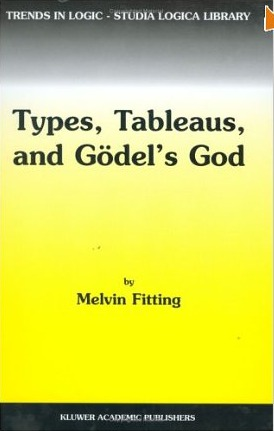
\includegraphics[height=2.5cm]{Images/Books/buch7.jpg}
} %$
\hfill
\colorbox{gray}{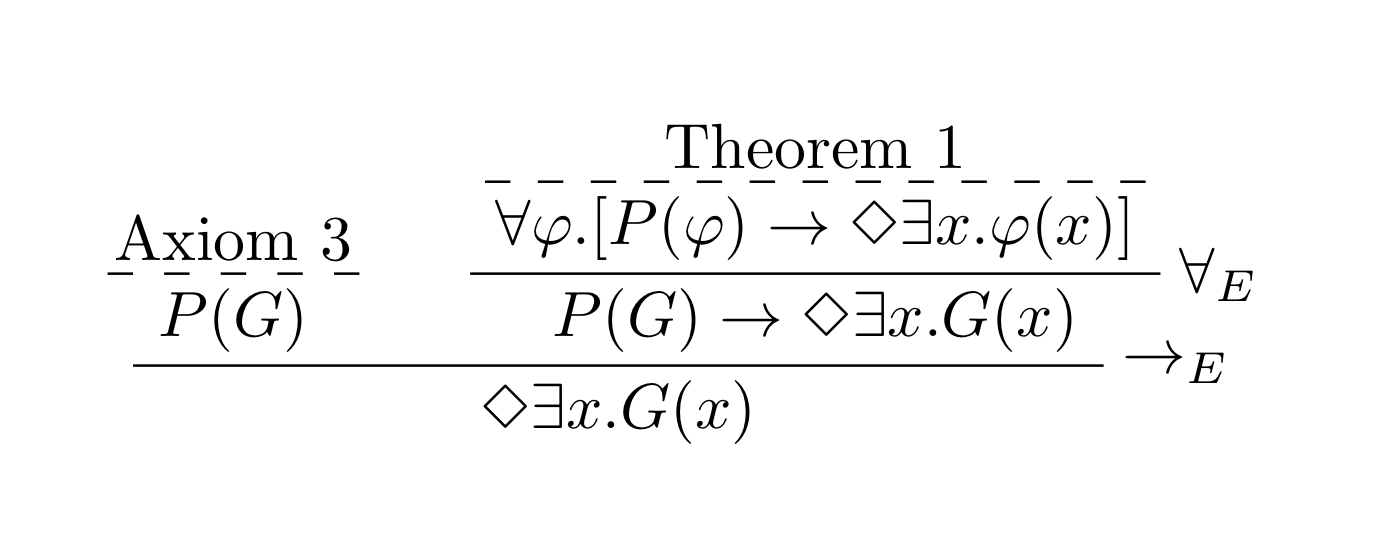
\includegraphics[height=2cm]{Images/ND.png}}%$

\hfill \begin{footnotesize}A gift to \textbf{Priest Edvaldo} in Piracicaba, Brazil\end{footnotesize}
\end{frame}

\author{\textbf{Christoph Benzm\"{u}ller} and \textbf{Bruno
    Woltzenlogel Paleo}}



\begin{frame}{Contribution}\Large
\colorbox{gray}{
\begin{minipage}{.9\textwidth} 
\textcolor{white}{First time mechanization and automation of}
\begin{itemize}
\item \textcolor{white}{(variants of) a modern ontological argument}
\item \textcolor{white}{(variants of) higher-order modal logic}
\end{itemize}
\end{minipage}
}
\vfill
Work context/history:\\[.2em]
\begin{itemize}
\item \textbf{Proposal:} exploit classical higher-order logic (HOL) as
  universal meta-logic --- cf. previous talks at UNILOG
  \begin{itemize}
  \item for object-level reasoning (in embedded non-classical logics)
  \item for meta-level reasoning (about embedded non-classical logics)
  \end{itemize}
\item \textbf{Proof of concept:} demonstrate practical relevance of the approach by
  an interesting and relevant application
\item \textbf{Experiments:} systematic study of G�del's argument
% \item Results: Verification  of known results / partly novel results
\item \textbf{Relation to Square of Opposition:} should be easy to analyze variants of the Square within our approach
\end{itemize}
\end{frame}



\begin{frame}{Introduction} \large
\hskip-1em \textbf{Challenge:} \hfill No provers for \emph{Higher-order Quantified Modal Logic\/} (\textcolor{red}{QML}) \\[1em]

\hskip-1em \textbf{Our solution:} \hfill Embedding in \emph{Higher-order Classical Logic\/} (\textcolor{blue}{HOL}) \\[1em]
%\,\hfill {\small [Benzm\"ullerPaulson, Logica Universalis, 2013]} \\[2em]

\hskip-1em \textbf{What we did:} \\

\begin{itemize}
\item[A:] Pen and paper: \hfill detailed natural deduction proof 
\item[B:] Formalization: \hfill in classical higher-order logic (\textcolor{blue}{HOL})
\item[] Automation: \hfill theorem provers \textsc{LEO-II(\textbf{E})} and \textsc{Satallax} 
\item[] Consistency: \hfill model finder \textsc{Nitpick (Nitrox)} 
\item[C:] Step-by-step verification: \hfill proof assistant \textsc{Coq} 
\item[D:] Automation \& verification: \hfill proof assistant \textsc{Isabelle} \\[2em]
%\item[ ] Conclusion \\[2em]
\end{itemize}
\hskip-1em  \textbf{Did we get any new results? }\hfill  \textcolor{red}{Yes --- let's discuss this later!}
\end{frame}



\begin{frame}{Introduction} \small
\vskip1em
\begin{minipage}{.56\textwidth} 
\onslide*<1-2>{
\onslide*<1>{\colorbox{gray}{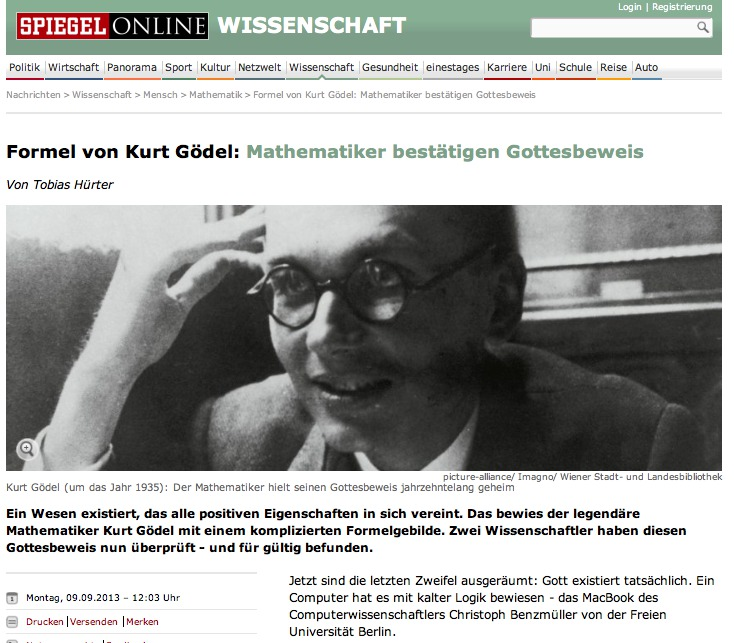
\includegraphics[width=.95\textwidth]{Images/News/spiegel1}}}%
\onslide*<2>{\colorbox{gray}{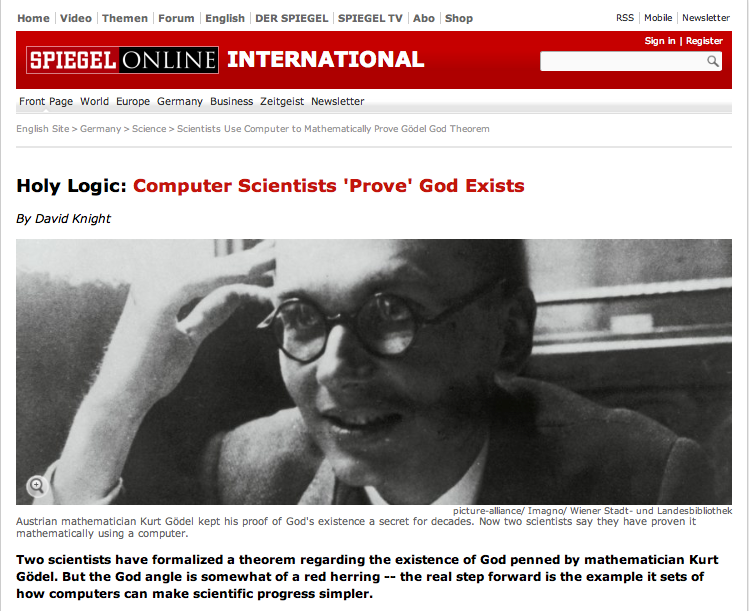
\includegraphics[width=\textwidth]{Images/News/spiegel2}}}%$
\vskip1em
Germany \\
- Telepolis \& Heise \\
- Spiegel Online \\
- FAZ \\
- Die Welt \\
- Berliner Morgenpost \\
- Hamburger Abendpost \\
- \ldots \\
}
%\onslide*<3>{\colorbox{gray}{
\includegraphics[width=\textwidth]{Images/News/welt}}}
\end{minipage} \hfill
%
\begin{minipage}{.3\textwidth}
Austria \\
- Die Presse \\
- Wiener Zeitung \\
- ORF \\
- \ldots \\

Italy \\
- Repubblica \\
- Ilsussidario \\
- \ldots \\

% Russia \\
% - \ldots \\

India \\
- DNA India \\
- Delhi Daily News \\
- India Today \\
- \ldots \\

US \\
- ABC News \\
- \ldots \\

International \\
- Spiegel International \\
- Yahoo Finance \\
% - CNET \\
- United Press Intl. \\
- \ldots \\
\end{minipage}
\end{frame}

\begin{frame}{Introduction} \large
\colorbox{gray}{
\includegraphics[width=\textwidth]{Images/News/MacBookGrab}} %$
\pause
\vfill
% Are we in contact with Steve Jobs? \hfill No \\[2em]
Do you really need a MacBook to obtain the results? \hfill No \\[2em]
Did Apple send us some money? \hfill No \\
%\, \hfill (but maybe they should)
\end{frame}



\begin{frame}{Introduction} \Large
\textbf{Rich history on ontological arguments} (\textcolor{blue}{pros} and \textcolor{red}{cons})\\[1em]

\hskip-.5em
\ldots\rotatebox[origin = bl,width = 0mm]{65}{\textcolor{blue}{Anselm v. C.}} \hskip-2.3em
          \rotatebox[origin = bl]{65}{\textcolor{red}{Gaunilo}} \hskip-1.3em
\ldots  \rotatebox[origin = bl]{65}{\textcolor{red}{Th. Aquinas}}  \hskip-2.3em
\ldots\ldots   \rotatebox[origin = bl]{65}{\textcolor{blue}{Descartes}} \hskip-1.7em
               \rotatebox[origin = bl]{65}{\textcolor{blue}{Spinoza}} \hskip-1.3em
               \rotatebox[origin = bl]{65}{\textcolor{blue}{Leibniz}}  \hskip-1.2em
\ldots  \rotatebox[origin = bl]{65}{\textcolor{red}{Hume}}  \hskip-1em
          \rotatebox[origin = bl]{65}{\textcolor{red}{Kant}}  \hskip-.8em
\ldots  \rotatebox[origin = bl]{65}{\textcolor{blue}{Hegel}}  \hskip-1.3em
\ldots  \rotatebox[origin = bl]{65}{\textcolor{red}{Frege}}  \hskip-1.3em
\ldots  \rotatebox[origin = bl]{65}{\textcolor{blue}{Hartshorne}} \hskip-1.9em
          \rotatebox[origin = bl]{65}{\textcolor{blue}{Malcolm}}  \hskip-1.4em
          \rotatebox[origin = bl]{65}{\textcolor{red}{Lewis}}  \hskip-1em
          \rotatebox[origin = bl]{65}{\textcolor{blue}{Plantinga}}  \hskip-1.6em
          \rotatebox[origin = bl]{65}{\textcolor{blue}{G\"odel}}   \hskip-1.2em
\ldots \\[1em]

\pause
\vfill
\textbf{Anselm's notion of God:}\\
\,\hfill \emph{``God is that, than which nothing greater can be
  conceived.''} \\[1em]

\textbf{G\"odel's notion of God:}\\
\,\hfill \emph{``A God-like being possesses all `positive' properties.''} \\[1em]

\textbf{To show by logical reasoning:} \\
\,\hfill \emph{``(Necessarily) God exists.''} \\[1em]

% \rnode{n2}{}\emph{}
% \ncline[nodesep=2pt,linecolor=black,linewidth=1pt]{->}{n1}{n2}
\end{frame}


\begin{frame}{Introduction} \Large
\textbf{Different Interests in Ontological Arguments:} \\[1em]
\begin{itemize}
\item \textcolor{blue}{Philosophical:} Boundaries of Metaphysics \& Epistemology
  \begin{itemize}
  \item We talk about a metaphysical concept (God), 
  \item but we want to draw
      a conclusion for the real world. % \\[1em]
 % \item Necessary Existence: metaphysical NE vs. logical NE  vs. modal NE 
   \\[2em]
  \end{itemize} 
\item \textcolor{blue}{Theistic:} Successful argument should convince atheists \\[2em]
\item \textcolor{red}{Ours:} Can computers (theorem provers) be used \ldots
  \begin{itemize}
  \item \ldots to formalize the definitions, axioms and theorems?
  \item \ldots to verify the arguments step-by-step?
  \item \ldots to fully automate (sub-)arguments? \\[2em]
  \end{itemize}
  Towards: \textcolor{red}{\emph{`Computer-assisted Theoretical
      Philosophy''}} \\[.5cm]
  (cf. Leibniz dictum --- Calculemus!) \\
 % (cf. the Computational Metaphysics Project at Stanford University)
\end{itemize}
\end{frame}



\begin{frame}{G\"odel's Manuscript: 1930's, 1941, 1946-1955, 1970}
\bigskip

\begin{changemargin}{-1.2cm}{-1.2cm}
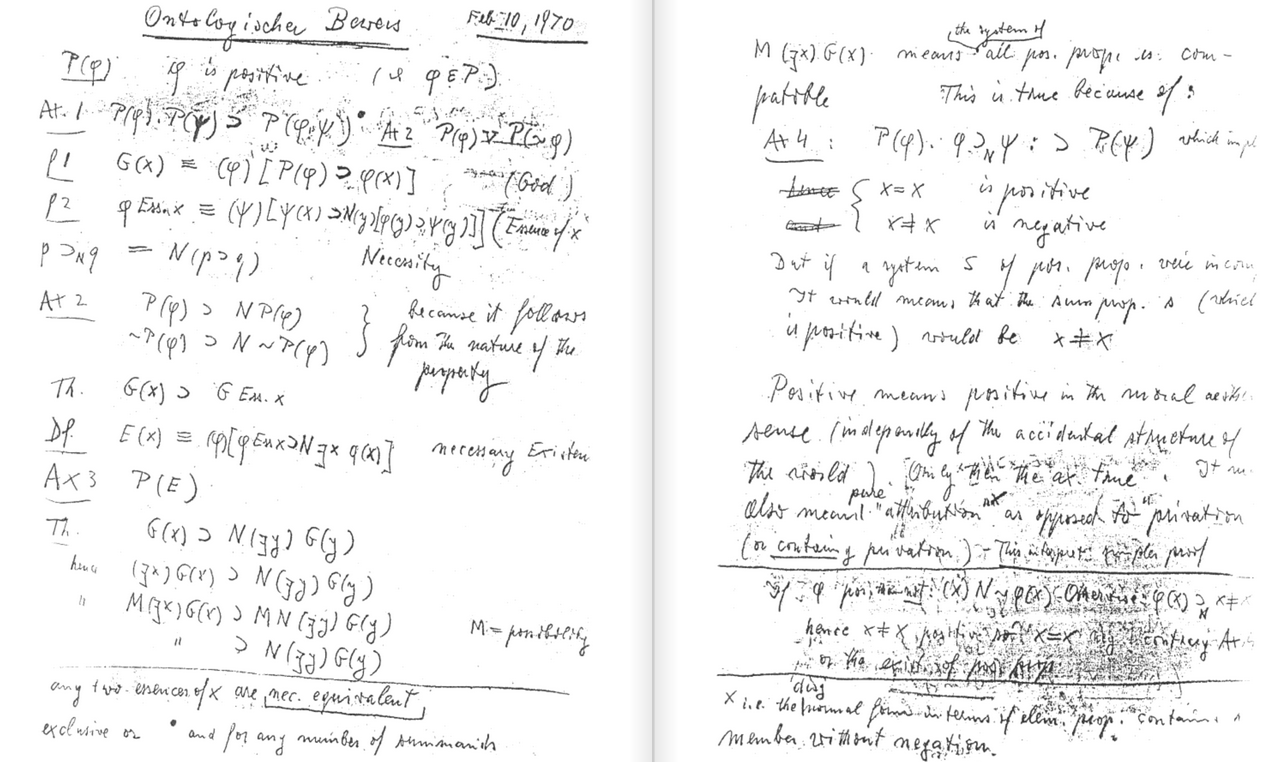
\includegraphics[width=13cm]{Images/Manuscript.png}%$
\end{changemargin}
\end{frame}

\begin{frame}{Scott's Version of G\"odel's Axioms, Definitions and
    Theorems}
\scottproof
\end{frame}


\begin{frame}{Remainder of this Talk}\Large
\begin{itemize}
\item Embedding of \textcolor{red}{QML} in \textcolor{blue}{HOL} and
  Proof Automation (myself) \\[1em]
\item Proof Overview (Bruno)
\item Experiments and Results (Bruno)
\item Conclusion and Outlook (Bruno)
\end{itemize}
\end{frame}



\begin{transitionframe}{Images/Transitions/GodComputerC}{black} %$
\textbf{Embedding of \textcolor{red}{QML} in \textcolor{blue}{HOL}  and Proof Automation} \\[.5em]
% \quad Formalization: \hfill in classical higher-order logic (\textcolor{black}{HOL}) \\
% \quad Automation: \hfill theorem provers \textsc{Leo-II} and \textsc{Satallax} \\ 
% \quad Consistency: \hfill model finder \textsc{Nitpick (Nitrox)} \\
\end{transitionframe}

\begin{frame}{Formalization in HOL} \large

\hskip-1em \textbf{Challenge:} \hfill No provers for \emph{Higher-order
  Quantified Modal
  Logic\/} (\textcolor{red}{QML}) \\[1em]

\hskip-1em \textbf{Our solution:} \hfill Embedding in \emph{Higher-order Classical
  Logic\/} (\textcolor{blue}{HOL}) \\
\, \hfill Then use existing \textcolor{blue}{HOL} theorem provers for reasoning in \textcolor{red}{QML} \\
\,\hfill {\small [Benzm\"ullerPaulson, Logica Universalis, 2013]}
\\[2em]

\hskip-1em \textbf{Previous empirical findings:}  \\[.5em]
\,\hfill Embedding of  \emph{First-order Modal Logic} in HOL works well 

\,\hfill {\small [Benzm\"ullerOttenRaths, ECAI, 2012]} \\
\,\hfill {\small [Benzm\"ullerRaths, LPAR, 2013]}
\end{frame}



\begin{frame}{Formalization in HOL} \large

\hskip-1em\textcolor{red}{QML} \hfill
$\begin{array}{lll}\textcolor{red}{\varphi,\psi} & ::= &
  \textcolor{red}{\ldots}  \mid \textcolor{red}{\neg
    \varphi} \mid \textcolor{red}{\varphi \wedge \psi} \mid
  \textcolor{red}{\varphi \imp \psi}  \mid \textcolor{red}{\Box
    \varphi} \mid \textcolor{red}{\Diamond \varphi}  \mid
  \textcolor{red}{\forall {x}\, \varphi} \mid
  \textcolor{red}{\exists {x}\, \varphi} 
\mid \textcolor{red}{\forall {P}\, \varphi} \end{array}$ \\[1em]


\begin{itemize}
\item Kripke style semantics (possible world semantics)\\[2em]
\end{itemize}



\hskip-1em\textcolor{blue}{HOL}\hfill 
$\begin{array}{lll}
\textcolor{blue}{s,t} & ::= & \textcolor{blue}{C}  \mid
\textcolor{blue}{x \mid \lambda{x} s} \mid \textcolor{blue}{s\, t}
\mid \textcolor{blue}{\neg s} \mid \textcolor{blue}{s \vee t} \mid
\textcolor{blue}{\forall {x}\, t} 
\end{array}$ \\[1em]

\begin{itemize}
\item meanwhile very well understood
\item \textbf{Henkin semantics} vs. standard semantics
\item various theorem provers do exist \\[.5em]
  \quad interactive: \hfill Isabelle/HOL, HOL4, Hol Light, Coq/HOL, PVS,
  \ldots \\[.5em]
  \quad automated: \hfill TPS, LEO-II, Satallax, Nitpick, Isabelle/HOL, \ldots \\
\end{itemize}


\end{frame}


\begin{frame}{Formalization in HOL}\large

\hskip-1em\textcolor{red}{QML} \hfill
$\begin{array}{lll}\textcolor{red}{\varphi,\psi} & ::= &
  \textcolor{red}{\ldots}  \mid \textcolor{red}{\neg
    \varphi} \mid \textcolor{red}{\varphi \wedge \psi} \mid
  \textcolor{red}{\varphi \imp \psi}  \mid \textcolor{red}{\Box
    \varphi} \mid \textcolor{red}{\Diamond \varphi}  \mid
  \textcolor{red}{\forall {x}\, \varphi} \mid
  \textcolor{red}{\exists {x}\, \varphi} 
\mid \textcolor{red}{\forall {P}\, \varphi} \end{array}$ \\[1em]

\hskip-1em\textcolor{blue}{HOL}\hfill 
$\begin{array}{lll}
\textcolor{blue}{s,t} & ::= & \textcolor{blue}{C}  \mid
\textcolor{blue}{x \mid \lambda{x} s} \mid \textcolor{blue}{s\, t}
\mid \textcolor{blue}{\neg s} \mid \textcolor{blue}{s \vee t} \mid
\textcolor{blue}{\forall {x}\, t} 
\end{array}$ \\[1em]

\pause

\hskip-1em\textcolor{red}{QML} in \textcolor{blue}{HOL}: \quad \textcolor{red}{QML}
formulas $\textcolor{red}{\varphi}$ are mapped to
\textcolor{blue}{HOL} predicates $\textcolor{red}{\varphi_{\worldtype\typearrow o}}$

\begin{center}
\fcolorbox{blue}{white}{
$\begin{array}{lcl} 
    \textcolor{red}{\mnot} & = & \textcolor{blue}{
      \lambda{\varphi_{\worldtype\typearrow o}}\lambda{s_\worldtype}\neg \varphi s} \\ 
    \textcolor{red}{\mand} & = & \textcolor{blue}{ 
      \lambda{\varphi_{\worldtype\typearrow o}}
      \lambda{\psi_{\worldtype\typearrow o}} \lambda{s_\worldtype}
      (\varphi s \wedge \psi s)} \\ 
    \textcolor{red}{\imp} & = & \textcolor{blue}{ 
      \lambda{\varphi_{\worldtype\typearrow o}}
      \lambda{\psi_{\worldtype\typearrow o}} \lambda{s_\worldtype}
      (\neg \varphi s \vee \psi s)} \\ 
    \textcolor{red}{\Box} & = & \textcolor{blue}{ 
      \lambda{\varphi_{\worldtype\typearrow o}} \lambda{s_\worldtype}
      \forall {u_\worldtype}\, (\neg r s u \vee
      \varphi u)} \\ 
    \textcolor{red}{\Diamond} & = & \textcolor{blue}{ 
      \lambda{\varphi_{\worldtype\typearrow o}} \lambda{s_\worldtype}
      \exists {u_\worldtype}\, (r s u \wedge
      \varphi u)} \\ 
    \textcolor{red}{\forall} & = & \textcolor{blue}{ 
      \lambda{h_{\mu\typearrow(\worldtype \typearrow o)}}
      \lambda{s_\worldtype} \forall {d_\indtype} \, h d s} \\
    \textcolor{red}{\exists} & = & \textcolor{blue}{ 
      \lambda{h_{\mu\typearrow(\worldtype \typearrow o)}}
      \lambda{s_\worldtype} \exists {d_\indtype} \, h d s} \\
    \textcolor{red}{\forall} & = & \textcolor{blue}{ 
      \lambda{H_{(\mu\typearrow(\worldtype \typearrow o))\typearrow(\worldtype \typearrow o)}}
      \lambda{s_\worldtype} \forall {d_\indtype} \, H d s} \\
    \\
      \text{\textcolor{brown}{valid}} & = & \textcolor{blue}{
        \lambda{\varphi_{\worldtype\typearrow o}} \all{w_\worldtype}
        \varphi w}
\end{array}$
}  \quad \textcolor{blue}{Ax} 
\vskip1em
\end{center}

\pause

\quad The equations in \textcolor{blue}{Ax} are given as axioms to the \textcolor{blue}{HOL} provers! \\
\quad \textcolor{gray}{\small (Remark: Note that we are here dealing with constant domain quantification)}

\end{frame}



\begin{frame}{Formalization in HOL} \large

\hskip-1em \textbf{Example:} \\[.5em]

 \textcolor{red}{QML} formula  \hfill \textcolor{red}{$\Diamond \exists x G(x)$}

\pause 

 \textcolor{red}{QML} formula in \textcolor{blue}{HOL}  \hfill $\text{\textcolor{brown}{valid}}\, \textcolor{red}{(\Diamond \exists x G(x))_{\worldtype\typearrow o}}$

\pause

expansion, $\beta\eta$-conversion \hfill $\textcolor{blue}{\forall
  w_\worldtype\textcolor{red}{(\Diamond \exists x
    G(x))_{\worldtype\typearrow o}}\, w}$ 

\pause

expansion, $\beta\eta$-conversion \hfill $\textcolor{blue}{\forall
  w_\worldtype \exists {u_\worldtype} (r w u \wedge
      \textcolor{red}{(\exists x G(x))_{\worldtype\typearrow o}} u)}$ 

% expansion, $\beta\eta$-conversion \hfill $\textcolor{blue}{\forall
%   w_\worldtype \exists {u_\worldtype} (r w u \wedge
%       \exists x \textcolor{red}{G(x)_{\worldtype\typearrow o}} u)}$ 

\pause

expansion, $\beta\eta$-conversion \hfill $\textcolor{blue}{\forall
  w_\worldtype \exists {u_\worldtype} (r w u \wedge
      \exists x G x u)}$ \\[1em]

\pause

\vfill
\begin{block}{What are we doing?}
\vskip.5em
In order to prove that $\textcolor{red}{\varphi}$ is valid in \textcolor{red}{QML}, \\
--> we instead prove that 
$\text{\textcolor{brown}{valid}}\,
\textcolor{red}{\varphi_{\worldtype\typearrow o}}$ can be derived
from \textcolor{blue}{Ax} in \textcolor{blue}{HOL}. \\[1em]

This can be done with interactive or automated \textcolor{blue}{HOL} theorem provers.
\end{block}
\pause
%\vfill
%\hskip-1em Expansion: \hfill user or prover may flexibly choose expansion depth \\[.5em]
\vfill
\hskip-1em \textbf{Soundness and Completeness:} \hfill wrt. Henkin semantics \\[.5em]
\end{frame}


\begin{frame}{Automated Theorem Provers and Model Finders for HOL}
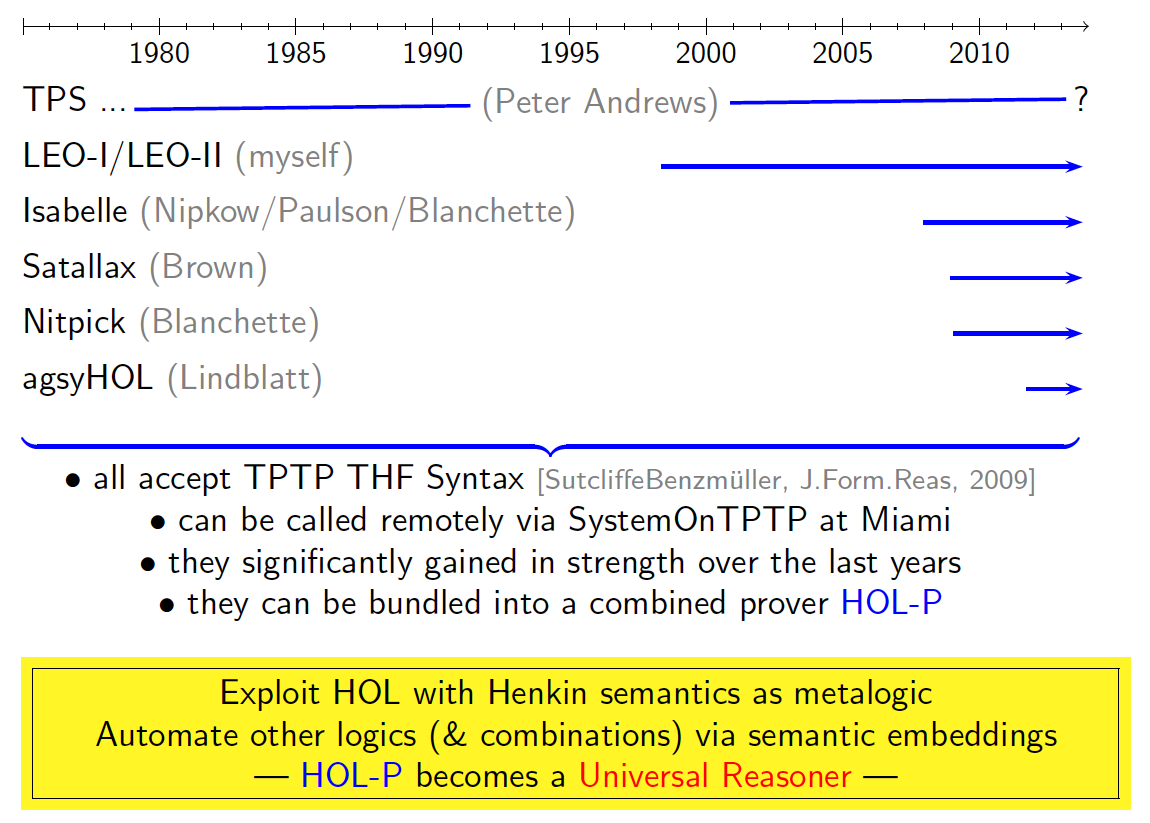
\includegraphics[width=1.05\textwidth]{Images/HOLProversGrab}%$
\end{frame}


\begin{transitionframe}{Images/Transitions/RioChrist3}{black}%$
\textbf{Proof Overview}\\
\textbf{Experiments and Results}
\end{transitionframe}

\begin{frame}{G\"odel's Manuscript: 1930's, 1941, 1946-1955, 1970}
\bigskip

\begin{changemargin}{-1.2cm}{-1.2cm}
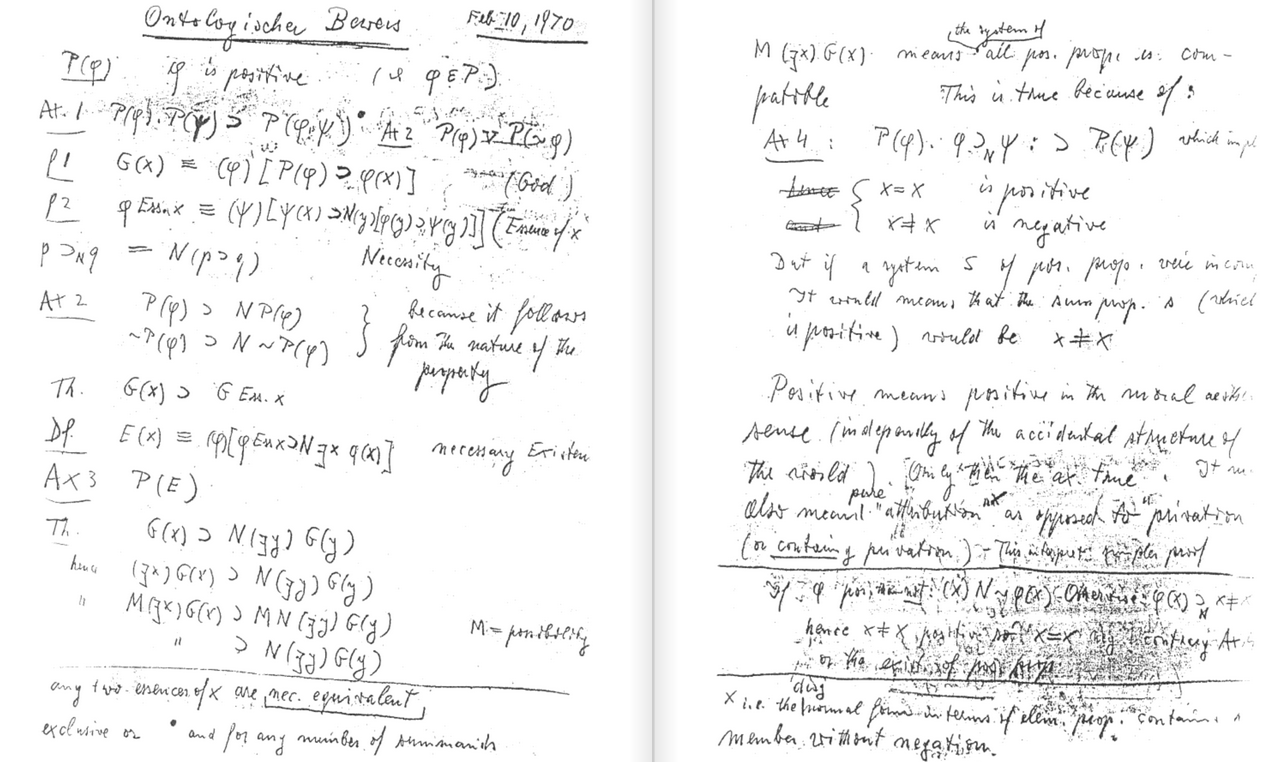
\includegraphics[width=13cm]{Images/Manuscript.png}%$
\end{changemargin}
\end{frame}

% \begin{frame}{Scott's Version of G\"odel's Axioms, Definitions and
%     Theorems}
% \scottproof
% \end{frame}



\newcommand{\phantomCOne}{
\begin{prooftree}
\AXC{$\phantom{\textbf{A3}}$} \noLine
\UIC{$\phantom{P(G)}$}
		\AXC{$\phantom{\textbf{A2}}$} \noLine
		\UIC{$\phantom{\all \varphi. \all \psi.[(P(\varphi) \wedge \nec \all x.[\varphi(x) \imp \psi(x)]) \imp P(\psi)]}$}
					\AXC{$\phantom{\textbf{A1a}}$} \noLine
					\UIC{$\phantom{\all \varphi. [P(\neg \varphi) \imp \neg P(\varphi)]}$} \noLine
				\BIC{$\phantom{\textbf{T1: } \all \varphi. [P(\varphi) \imp \pos \ex x.\varphi(x)]}$} \noLine
	\BIC{$\phantom{\textbf{C1: } \pos \ex z. G(z)}$}
\end{prooftree}
}

\newcommand{\phantomTTwo}{
\begin{prooftree}
						\AXC{$\phantom{\textbf{A1b}}$} \noLine
						\UIC{$\phantom{\all \varphi. [\neg P(\varphi) \imp P(\neg \varphi)]}$}
								\AXC{$\phantom{\textbf{A4}}$} \noLine
								\UIC{$\phantom{ \all \varphi.[P(\varphi) \to \Box \; P(\varphi)]} $} \noLine
							\BIC{$\phantom{\textbf{T2: } \all y.[G(y) \imp \ess{G}{y}]}$}
									\AXC{$\phantom{\textbf{A5}}$} \noLine
									\UIC{$ \phantom{P(E)} $} \noLine
								\BIC{$\phantom{\textbf{L1: } \ex z. G(z) \imp \nec \ex x. G(x)}$} \noLine
								\UIC{$\phantom{\pos \ex z. G(z) \imp \pos \nec \ex x. G(x)}$}
										\AXC{$\phantom{\textbf{S5}}$} \noLine
 										\UIC{$\phantom{\all \xi.[\pos \nec \xi \imp \nec \xi]}$} \noLine	
									\BIC{$\phantom{\textbf{L2: } \pos \ex z. G(z) \imp \nec \ex x. G(x)}$}
\end{prooftree}
}

\newcommand{\phantomDOne}{
$$
\phantom{
\textbf{D1: } G(x) \equiv \forall \varphi. [P(\varphi) \imp \varphi(x)]}
$$
}

\newcommand{\DOne}{
$$
\textbf{D1: } G(x) \equiv \forall \varphi. [P(\varphi) \imp \varphi(x)]
$$
}

\newcommand{\phantomDTwo}{
$$
\phantom{
\textbf{D2: } \ess{\varphi}{x} \equiv \varphi(x) \wedge \all \psi. (\psi(x) \imp \nec \all x. (\varphi(x) \imp \psi(x)))
}
$$
}

\newcommand{\DTwo}{
$$
\textbf{D2: } \ess{\varphi}{x} \equiv \textcolor{blue}{\varphi(x)} \wedge \all \psi. (\psi(x) \imp \nec \all x. (\varphi(x) \imp \psi(x)))
$$
}


\newcommand{\phantomDThree}{
$$
\phantom{
\textbf{D3: } E(x) \equiv \all \varphi.[\ess{\varphi}{x} \imp \nec \ex y.\varphi(y)]
}
$$
}

\newcommand{\DThree}{
$$
\textbf{D3: } E(x) \equiv \all \varphi.[\ess{\varphi}{x} \imp \nec \ex y.\varphi(y)]
$$
}


\begin{frame}[shrink]{Proof Overview}

\phantomDOne

\phantomDTwo

\phantomDThree

\phantomCOne

\phantomTTwo

\begin{prooftree}
\AXC{$\phantom{\textbf{C1: } \pos \ex z. G(z)}$}
		\AXC{$\phantom{\textbf{L2: } \pos \ex z. G(z) \imp \nec \ex x. G(x)}$} \noLine
	\BIC{$\textbf{T3: } \nec \ex x. G(x) $}
\end{prooftree}

\end{frame}




\begin{frame}[shrink]{Proof Overview}

\phantomDOne

\phantomDTwo

\phantomDThree

\phantomCOne

\phantomTTwo

\begin{prooftree}
\AXC{$\textbf{C1: } \pos \ex z. G(z)$}
		\AXC{$\phantom{\textbf{L2: } \pos \ex z. G(z) \imp \nec \ex x. G(x)}$}
	\BIC{$\textbf{T3: } \nec \ex x. G(x) $}
\end{prooftree}

\end{frame}



\newcommand{\TThree}{
\begin{prooftree}
\AXC{$\textbf{C1: } \pos \ex z. G(z)$}
		\AXC{$\textbf{L2: } \pos \ex z. G(z) \imp \nec \ex x. G(x)$}
	\BIC{$\textbf{T3: } \nec \ex x. G(x) $}
\end{prooftree}	
}


\begin{frame}[shrink]{Proof Overview}

\phantomDOne

\phantomDTwo

\phantomDThree

\phantomCOne

\phantomTTwo

\TThree

\end{frame}


\begin{frame}[shrink]{Proof Overview}

\begin{center}
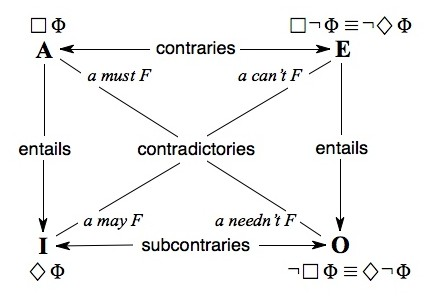
\includegraphics[width=\textwidth]{Images/ModalSquare}
\end{center}

\TThree

\end{frame}


\begin{frame}[shrink]{Proof Overview}

\phantomDOne

\phantomDTwo

\phantomDThree

\phantomCOne

\begin{prooftree}
						\AXC{$\phantom{\textbf{A1b}}$} \noLine
						\UIC{$\phantom{\all \varphi. [\neg P(\varphi) \imp P(\neg \varphi)]}$}
								\AXC{$\phantom{\textbf{A4}}$} \noLine
								\UIC{$\phantom{ \all \varphi.[P(\varphi) \to \Box \; P(\varphi)]} $} \noLine
							\BIC{$\phantom{\textbf{T2: } \all y.[G(y) \imp \ess{G}{y}]}$}
									\AXC{$\phantom{\textbf{A5}}$} \noLine
									\UIC{$ \phantom{P(E)} $} \noLine
								\BIC{$\phantom{\textbf{L1: } \ex z. G(z) \imp \nec \ex x. G(x)}$} \noLine
								\UIC{$\phantom{\pos \ex z. G(z) \imp \pos \nec \ex x. G(x)}$}
										\AXC{$\phantom{\textbf{S5}}$} \noLine
 										\UIC{$\phantom{\all \xi.[\pos \nec \xi \imp \nec \xi]}$} \noLine	
									\BIC{$\textbf{L2: } \pos \ex z. G(z) \imp \nec \ex x. G(x)$}
\end{prooftree}

\TThree

\end{frame}


\begin{frame}[shrink]{Proof Overview}

\phantomDOne

\phantomDTwo

\phantomDThree

\phantomCOne

\begin{prooftree}
						\AXC{$\phantom{\textbf{A1b}}$} \noLine
						\UIC{$\phantom{\all \varphi. [\neg P(\varphi) \imp P(\neg \varphi)]}$}
								\AXC{$\phantom{\textbf{A4}}$} \noLine
								\UIC{$\phantom{ \all \varphi.[P(\varphi) \to \Box \; P(\varphi)]} $} \noLine
							\BIC{$\phantom{\textbf{T2: } \all y.[G(y) \imp \ess{G}{y}]}$}
									\AXC{$\phantom{\textbf{A5}}$} \noLine
									\UIC{$ \phantom{P(E)} $} \noLine
								\BIC{$\phantom{\textbf{L1: } \ex z. G(z) \imp \nec \ex x. G(x)}$} \noLine
								\UIC{$\phantom{\pos \ex z. G(z) \imp \pos \nec \ex x. G(x)}$}
										\AXC{$\textbf{S5}$} \dashedLine
 										\UIC{$\all \xi.[\pos \nec \xi \imp \nec \xi]$} 	
									\BIC{$\textbf{L2: } \pos \ex z. G(z) \imp \nec \ex x. G(x)$}
\end{prooftree}

\TThree

\end{frame}




\begin{frame}[shrink]{Proof Overview}

\phantomDOne

\phantomDTwo

\phantomDThree

\phantomCOne

\begin{prooftree}
						\AXC{$\phantom{\textbf{A1b}}$} \noLine
						\UIC{$\phantom{\all \varphi. [\neg P(\varphi) \imp P(\neg \varphi)]}$}
								\AXC{$\phantom{\textbf{A4}}$} \noLine
								\UIC{$\phantom{ \all \varphi.[P(\varphi) \to \Box \; P(\varphi)]} $} \noLine
							\BIC{$\phantom{\textbf{T2: } \all y.[G(y) \imp \ess{G}{y}]}$}
									\AXC{$\phantom{\textbf{A5}}$} \noLine
									\UIC{$ \phantom{P(E)} $} \noLine
								\BIC{$\phantom{\textbf{L1: } \ex z. G(z) \imp \nec \ex x. G(x)}$} \noLine
								\UIC{$\pos \ex z. G(z) \imp \pos \nec \ex x. G(x)$}
										\AXC{$\textbf{S5}$} \dashedLine
 										\UIC{$\all \xi.[\pos \nec \xi \imp \nec \xi]$} 	
									\BIC{$\textbf{L2: } \pos \ex z. G(z) \imp \nec \ex x. G(x)$}
\end{prooftree}

\TThree

\end{frame}




\begin{frame}[shrink]{Proof Overview}

\phantomDOne

\phantomDTwo

\phantomDThree

\phantomCOne

\begin{prooftree}
						\AXC{$\phantom{\textbf{A1b}}$} \noLine
						\UIC{$\phantom{\all \varphi. [\neg P(\varphi) \imp P(\neg \varphi)]}$}
								\AXC{$\phantom{\textbf{A4}}$} \noLine
								\UIC{$\phantom{ \all \varphi.[P(\varphi) \to \Box \; P(\varphi)]} $} \noLine
							\BIC{$\phantom{\textbf{T2: } \all y.[G(y) \imp \ess{G}{y}]}$}
									\AXC{$\phantom{\textbf{A5}}$} \noLine
									\UIC{$ \phantom{P(E)} $} \noLine
								\BIC{$\textbf{L1: } \ex z. G(z) \imp \nec \ex x. G(x)$} 
								\UIC{$\pos \ex z. G(z) \imp \pos \nec \ex x. G(x)$}
										\AXC{$\textbf{S5}$} \dashedLine
 										\UIC{$\all \xi.[\pos \nec \xi \imp \nec \xi]$} 	
									\BIC{$\textbf{L2: } \pos \ex z. G(z) \imp \nec \ex x. G(x)$}
\end{prooftree}

\TThree

\end{frame}



\begin{frame}[shrink]{Proof Overview}

\DOne

\phantomDTwo

\phantomDThree

\phantomCOne

\begin{prooftree}
						\AXC{$\phantom{\textbf{A1b}}$} \noLine
						\UIC{$\phantom{\all \varphi. [\neg P(\varphi) \imp P(\neg \varphi)]}$}
								\AXC{$\phantom{\textbf{A4}}$} \noLine
								\UIC{$\phantom{ \all \varphi.[P(\varphi) \to \Box \; P(\varphi)]} $} \noLine
							\BIC{$\phantom{\textbf{T2: } \all y.[G(y) \imp \ess{G}{y}]}$}
									\AXC{$\phantom{\textbf{A5}}$} \noLine
									\UIC{$ \phantom{P(E)} $} \noLine
								\BIC{$\textbf{L1: } \ex z. G(z) \imp \nec \ex x. G(x)$} 
								\UIC{$\pos \ex z. G(z) \imp \pos \nec \ex x. G(x)$}
										\AXC{$\textbf{S5}$} \dashedLine
 										\UIC{$\all \xi.[\pos \nec \xi \imp \nec \xi]$} 	
									\BIC{$\textbf{L2: } \pos \ex z. G(z) \imp \nec \ex x. G(x)$}
\end{prooftree}

\TThree

\end{frame}


% \begin{frame}[shrink]{Proof Overview}

% \DOne

% \phantomDTwo

% \qquad
% \alert{$\textbf{D3*: } E(x) \equiv \nec \ex y. G(y)$} \only<2>{(cheating!)}

% \phantomCOne

% \begin{prooftree}
% 						\AXC{$\phantom{\textbf{A1b}}$} \noLine
% 						\UIC{$\phantom{\all \varphi. [\neg P(\varphi) \imp P(\neg \varphi)]}$}
% 								\AXC{$\phantom{\textbf{A4}}$} \noLine
% 								\UIC{$\phantom{ \all \varphi.[P(\varphi) \to \Box \; P(\varphi)]} $} \noLine
% 							\BIC{$\phantom{\textbf{T2: } \all y.[G(y) \imp \ess{G}{y}]}$}
% 									\AXC{$\phantom{\textbf{A5}}$} \noLine
% 									\UIC{$ P(E) $}
% 								\BIC{$\textbf{L1: } \ex z. G(z) \imp \nec \ex x. G(x)$} 
% 								\UIC{$\pos \ex z. G(z) \imp \pos \nec \ex x. G(x)$}
% 										\AXC{$\textbf{S5}$} \dashedLine
%  										\UIC{$\all \xi.[\pos \nec \xi \imp \nec \xi]$} 	
% 									\BIC{$\textbf{L2: } \pos \ex z. G(z) \imp \nec \ex x. G(x)$}
% \end{prooftree}

% \TThree

% \end{frame}


\begin{frame}[shrink]{Proof Overview}

\DOne

\phantomDTwo


$$\textbf{D3: } E(x) \equiv \all \varphi.[\ess{\varphi}{x} \imp \nec \ex y.\varphi(y)]$$

\phantomCOne

\begin{prooftree}
						\AXC{$\phantom{\textbf{A1b}}$} \noLine
						\UIC{$\phantom{\all \varphi. [\neg P(\varphi) \imp P(\neg \varphi)]}$}
								\AXC{$\phantom{\textbf{A4}}$} \noLine
								\UIC{$\phantom{ \all \varphi.[P(\varphi) \to \Box \; P(\varphi)]} $} \noLine
							\BIC{$\textbf{T2: } \all y.[G(y) \imp \ess{G}{y}]$}
									\AXC{$\phantom{\textbf{A5}}$} \noLine
									\UIC{$ P(E) $}
								\BIC{$\textbf{L1: } \ex z. G(z) \imp \nec \ex x. G(x)$} 
								\UIC{$\pos \ex z. G(z) \imp \pos \nec \ex x. G(x)$}
										\AXC{$\textbf{S5}$} \dashedLine
 										\UIC{$\all \xi.[\pos \nec \xi \imp \nec \xi]$} 	
									\BIC{$\textbf{L2: } \pos \ex z. G(z) \imp \nec \ex x. G(x)$}
\end{prooftree}

\TThree

\end{frame}


\begin{frame}[shrink]{Proof Overview}

\DOne

\phantomDTwo

% \qquad
% \alert{$\textbf{D3*: } E(x) \equiv \nec \ex y. G(y)$}
% \qquad\qquad
$$\textbf{D3: } E(x) \equiv \all \varphi.[\ess{\varphi}{x} \imp \nec \ex y.\varphi(y)]$$
\phantomCOne

\begin{prooftree}
						\AXC{$\phantom{\textbf{A1b}}$} \noLine
						\UIC{$\phantom{\all \varphi. [\neg P(\varphi) \imp P(\neg \varphi)]}$}
								\AXC{$\phantom{\textbf{A4}}$} \noLine
								\UIC{$\phantom{ \all \varphi.[P(\varphi) \to \Box \; P(\varphi)]} $} \noLine
							\BIC{$\textbf{T2: } \all y.[G(y) \imp \ess{G}{y}]$}
									\AXC{$\textbf{A5}$} \dashedLine
									\UIC{$ P(E) $}
								\BIC{$\textbf{L1: } \ex z. G(z) \imp \nec \ex x. G(x)$} 
								\UIC{$\pos \ex z. G(z) \imp \pos \nec \ex x. G(x)$}
										\AXC{$\textbf{S5}$} \dashedLine
 										\UIC{$\all \xi.[\pos \nec \xi \imp \nec \xi]$} 	
									\BIC{$\textbf{L2: } \pos \ex z. G(z) \imp \nec \ex x. G(x)$}
\end{prooftree}

\TThree

\end{frame}



\begin{frame}[shrink]{Proof Overview}

\DOne

\phantomDTwo

% \qquad
% \alert{$\textbf{D3*: } E(x) \equiv \nec \ex y. G(y)$}
% \qquad\qquad
$$\textbf{D3: } E(x) \equiv \all \varphi.[\ess{\varphi}{x} \imp \nec \ex y.\varphi(y)]$$
\phantomCOne

\begin{prooftree}
						\AXC{$\phantom{\textbf{A1b}}$} \noLine
						\UIC{$\phantom{\all \varphi. [\neg P(\varphi) \imp P(\neg \varphi)]}$}
								\AXC{$\phantom{\textbf{A4}}$} \noLine
								\UIC{$\phantom{ \all \varphi.[P(\varphi) \to \Box \; P(\varphi)]} $} \noLine
							\BIC{$\textbf{T2: } \all y.[G(y) \imp \ess{G}{y}]$}
									\AXC{$\textbf{A5}$} \dashedLine
									\UIC{$ P(E) $}
								\BIC{$\textbf{L1: } \ex z. G(z) \imp \nec \ex x. G(x)$} 
								\UIC{$\pos \ex z. G(z) \imp \pos \nec \ex x. G(x)$}
										\AXC{$\textbf{S5}$} \dashedLine
 										\UIC{$\all \xi.[\pos \nec \xi \imp \nec \xi]$} 	
									\BIC{$\textbf{L2: } \pos \ex z. G(z) \imp \nec \ex x. G(x)$}
\end{prooftree}

\TThree

\end{frame}


\newcommand{\LTwo}{
\begin{prooftree}
						\AXC{$\textbf{A1b}$} \dashedLine
						\UIC{$\all \varphi. [\neg P(\varphi) \imp P(\neg \varphi)]$}
								\AXC{$\textbf{A4}$} \dashedLine
								\UIC{$ \all \varphi.[P(\varphi) \to \Box \; P(\varphi)] $} 
							\BIC{$\textbf{T2: } \all y.[G(y) \imp \ess{G}{y}]$}
									\AXC{$\textbf{A5}$} \dashedLine
									\UIC{$ P(E) $}
								\BIC{$\textbf{L1: } \ex z. G(z) \imp \nec \ex x. G(x)$} 
								\UIC{$\pos \ex z. G(z) \imp \pos \nec \ex x. G(x)$}
										\AXC{$\textbf{S5}$} \dashedLine
 										\UIC{$\all \xi.[\pos \nec \xi \imp \nec \xi]$} 	
									\BIC{$\textbf{L2: } \pos \ex z. G(z) \imp \nec \ex x. G(x)$}
\end{prooftree}
}


\begin{frame}[shrink]{Proof Overview}

\DOne

\DTwo

% \qquad
% \alert{$\textbf{D3*: } E(x) \equiv \nec \ex y. G(y)$}
% \qquad\qquad
$$\textbf{D3: } E(x) \equiv \all \varphi.[\ess{\varphi}{x} \imp \nec \ex y.\varphi(y)]$$

\phantomCOne

\LTwo

\TThree

\end{frame}


\begin{frame}[shrink]{Proof Overview}

\DOne

\DTwo

% \qquad
% \alert{$\textbf{D3*: } E(x) \equiv \nec \ex y. G(y)$}
% \qquad\qquad
$$\textbf{D3: } E(x) \equiv \all \varphi.[\ess{\varphi}{x} \imp \nec \ex y.\varphi(y)]$$

\begin{prooftree}
\AXC{$\phantom{\textbf{A3}}$} \noLine
\UIC{$\phantom{P(G)}$}
		\AXC{$\phantom{\textbf{A2}}$} \noLine
		\UIC{$\phantom{\all \varphi. \all \psi.[(P(\varphi) \wedge \nec \all x.[\varphi(x) \imp \psi(x)]) \imp P(\psi)]}$}
					\AXC{$\phantom{\textbf{A1a}}$} \noLine
					\UIC{$\phantom{\all \varphi. [P(\neg \varphi) \imp \neg P(\varphi)]}$} \noLine
				\BIC{$\phantom{\textbf{T1: } \all \varphi. [P(\varphi) \imp \pos \ex x.\varphi(x)]}$} \noLine
	\BIC{$\textbf{C1: } \pos \ex z. G(z)$}
\end{prooftree}

\LTwo

\TThree

\end{frame}


% \begin{frame}[shrink]{Proof Overview}

% \DOne

% \DTwo

% % \qquad
% % \alert{$\textbf{D3*: } E(x) \equiv \nec \ex y. G(y)$}
% % \qquad\qquad
% $$\textbf{D3: } E(x) \equiv \all \varphi.[\ess{\varphi}{x} \imp \nec \ex y.\varphi(y)]$$

% \begin{prooftree}
% \AXC{$\phantom{\textbf{A3}}$} \noLine
% \UIC{$P(G)$}
% 		\AXC{$\phantom{\textbf{A2}}$} \noLine
% 		\UIC{$\phantom{\all \varphi. \all \psi.[(P(\varphi) \wedge \nec \all x.[\varphi(x) \imp \psi(x)]) \imp P(\psi)]}$}
% 					\AXC{$\phantom{\textbf{A1a}}$} \noLine
% 					\UIC{$\phantom{\all \varphi. [P(\neg \varphi) \imp \neg P(\varphi)]}$} \noLine
% 				\BIC{$\phantom{\textbf{T1: } \all \varphi. [P(\varphi) \imp \pos \ex x.\varphi(x)]}$} 
% 	\BIC{$\textbf{C1: } \pos \ex z. G(z)$}
% \end{prooftree}

% \LTwo

% \TThree

% \end{frame}


% \begin{frame}[shrink]{Proof Overview}

% \DOne

% \DTwo

% % \qquad
% % \alert{$\textbf{D3*: } E(x) \equiv \nec \ex y. G(y)$}
% % \qquad\qquad
% $$\textbf{D3: } E(x) \equiv \all \varphi.[\ess{\varphi}{x} \imp \nec \ex y.\varphi(y)]$$

% \begin{prooftree}
% \AXC{$\textbf{A3}$} \dashedLine
% \UIC{$P(G)$}
% 		\AXC{$\phantom{\textbf{A2}}$} \noLine
% 		\UIC{$\phantom{\all \varphi. \all \psi.[(P(\varphi) \wedge \nec \all x.[\varphi(x) \imp \psi(x)]) \imp P(\psi)]}$}
% 					\AXC{$\phantom{\textbf{A1a}}$} \noLine
% 					\UIC{$\phantom{\all \varphi. [P(\neg \varphi) \imp \neg P(\varphi)]}$} \noLine
% 				\BIC{$\phantom{\textbf{T1: } \all \varphi. [P(\varphi) \imp \pos \ex x.\varphi(x)]}$} 
% 	\BIC{$\textbf{C1: } \pos \ex z. G(z)$}
% \end{prooftree}

% \LTwo

% \TThree

% \end{frame}



\begin{frame}[shrink]{Proof Overview}

\DOne

\DTwo

% \qquad
% \alert{$\textbf{D3*: } E(x) \equiv \nec \ex y. G(y)$}
% \qquad\qquad
$$\textbf{D3: } E(x) \equiv \all \varphi.[\ess{\varphi}{x} \imp \nec \ex y.\varphi(y)]$$

\begin{prooftree}
\AXC{$\textbf{A3}$} \dashedLine
\UIC{$P(G)$}
		\AXC{$\phantom{\textbf{A2}}$} \noLine
		\UIC{$\phantom{\all \varphi. \all \psi.[(P(\varphi) \wedge \nec \all x.[\varphi(x) \imp \psi(x)]) \imp P(\psi)]}$}
					\AXC{$\phantom{\textbf{A1a}}$} \noLine
					\UIC{$\phantom{\all \varphi. [P(\neg \varphi) \imp \neg P(\varphi)]}$} \noLine
				\BIC{$\textbf{T1: } \all \varphi. [P(\varphi) \imp \pos \ex x.\varphi(x)]$} 
	\BIC{$\textbf{C1: } \pos \ex z. G(z)$}
\end{prooftree}

\LTwo

\TThree

\end{frame}



\begin{frame}[shrink]{Proof Overview}

\DOne

\DTwo

% \qquad
% \alert{$\textbf{D3*: } E(x) \equiv \nec \ex y. G(y)$}
% \qquad\qquad
$$\textbf{D3: } E(x) \equiv \all \varphi.[\ess{\varphi}{x} \imp \nec \ex y.\varphi(y)]$$

\begin{prooftree}
\AXC{$\textbf{A3}$} \dashedLine
\UIC{$P(G)$}
		\AXC{$\textbf{A2}$} \dashedLine
		\UIC{$\all \varphi. \all \psi.[(P(\varphi) \wedge \nec \all x.[\varphi(x) \imp \psi(x)]) \imp P(\psi)]$}
					\AXC{$\textbf{A1a}$} \dashedLine
					\UIC{$\all \varphi. [P(\neg \varphi) \imp \neg P(\varphi)]$}
				\BIC{$\textbf{T1: } \all \varphi. [P(\varphi) \imp \pos \ex x.\varphi(x)]$} 
	\BIC{$\textbf{C1: } \pos \ex z. G(z)$}
\end{prooftree}

\LTwo

\TThree

\end{frame}



\begin{frame}[shrink]{Proof Overview}

$$
\textbf{D1: } G(x) \equiv \forall \varphi. [P(\varphi) \to \varphi(x)]
$$

$$
\textbf{D2: } \ess{\varphi}{x} \equiv \varphi(x) \wedge \all \psi. (\psi(x) \imp \nec \all x. (\varphi(x) \imp \psi(x)))
$$

$$
\textbf{D3: } E(x) \equiv \all \varphi.[\ess{\varphi}{x} \imp \nec \ex y.\varphi(y)]
$$

\begin{prooftree}
\AXC{$\textbf{A3}$} \dashedLine
\UIC{$P(G)$}
		\AXC{$\textbf{A2}$} \dashedLine
		\UIC{$\all \varphi. \all \psi.[(P(\varphi) \wedge \nec \all x.[\varphi(x) \imp \psi(x)]) \imp P(\psi)]$}
					\AXC{$\textbf{A1a}$} \dashedLine
					\UIC{$\all \varphi. [P(\neg \varphi) \imp \neg P(\varphi)]$} \doubleLine
				\BIC{$\textbf{T1: } \all \varphi. [P(\varphi) \imp \pos \ex x.\varphi(x)]$} \doubleLine
	\BIC{$\textbf{C1: } \pos \ex z. G(z)$}
\end{prooftree}


\begin{prooftree}
						\AXC{$\textbf{A1b}$} \dashedLine
						\UIC{$\all \varphi. [\neg P(\varphi) \imp P(\neg \varphi)]$}
								\AXC{$\textbf{A4}$} \dashedLine
								\UIC{$ \all \varphi.[P(\varphi) \to \Box \; P(\varphi)] $} \doubleLine
							\BIC{$\textbf{T2: } \all y.[G(y) \imp \ess{G}{y}]$}
									\AXC{$\textbf{A5}$} \dashedLine
									\UIC{$ P(E) $} \doubleLine
								\BIC{$\textbf{L1: } \ex z. G(z) \imp \nec \ex x. G(x)$} \doubleLine
								\UIC{$\pos \ex z. G(z) \imp \pos \nec \ex x. G(x)$}
										\AXC{$\textbf{S5}$} \dashedLine
 										\UIC{$ \all \xi.[\pos \nec \xi \imp \nec \xi]$} \doubleLine	
									\BIC{$\textbf{L2: } \pos \ex z. G(z) \imp \nec \ex x. G(x)$}
\end{prooftree}

\begin{prooftree}
\AXC{$\textbf{C1: } \pos \ex z. G(z)$}
		\AXC{$\textbf{L2: } \pos \ex z. G(z) \imp \nec \ex x. G(x)$} \doubleLine
	\BIC{$\textbf{T3: } \nec \ex x. G(x) $}
\end{prooftree}

\end{frame}




\begin{frame}[shrink]{Natural Deduction Calculus}

\begin{unnamedCalculus}

\vspace{1em}

\s\s
\infer[\vee_E]{C}{A \vee B & \infer*{C}{\infer{A}{}} & \infer*{C}{\infer{B}{}}}
\s\s
\infer[\wedge_I]{A \wedge B}{A & B}
\s\s
\infer[\imp_I^n]{A \imp B}{ \infer*{B}{\infer[n]{A}{}} }

\vspace{2em}

\s\s
\infer[\vee_{I_1}]{A \vee B}{A}
\s\s
\infer[\wedge_{E_1}]{A}{A \wedge B}
\s\s
\infer[\imp_I]{A \imp B}{ B }

\vspace{2em}

\s\s
\infer[\vee_{I_2}]{A \vee B}{B}
\s\s
\infer[\wedge_{E_2}]{B}{A \wedge B}
\s\s
\infer[\imp_E]{B}{A & A \imp B}

\vspace{2em}

\s
\infer[\all_I]{\all x. A[x]}{ A[\alpha] }
\s
\infer[\all_E]{A[t]}{ \all x. A[x] }
\s\s
\infer[\ex_I]{\ex x. A[x]}{ A[t] }
\s
\infer[\ex_E]{A[\beta]}{ \ex x. A[x] }

\vspace{1em}

\s\s\s\s
$\neg A \equiv A \imp \bot$ 
\s\s\s 
\alert{\infer[\neg\neg_E]{A}{\neg\neg A}}

\vspace{1em}

\end{unnamedCalculus}

\end{frame}



\begin{frame}[shrink]{Natural Deduction Calculus}{Rules for Modalities}

\begin{unnamedCalculus}

\vspace{1em}

\s\s\s\s
\infer[\nec_I]{\nec A}{\alpha: \fbox{\infer*{A}{}} }
\s\s\s\s\s
\infer[\nec_E]{t: \fbox{ \infer*{}{A} }  }{\nec A}

\vspace{2em}

\s\s\s\s
\infer[\pos_I]{\pos A}{t: \fbox{\infer*{A}{}} }
\s\s\s\s\s
\infer[\pos_E]{\beta: \fbox{ \infer*{}{A} }  }{\pos A}

\vspace{2em}

\alert{$$\pos A \equiv \neg \nec \neg A$$}

\vspace{1em}

\end{unnamedCalculus}

\end{frame}


% \begin{frame}[shrink]{Natural Deduction Calculus}{Three tiny examples}

% \vspace{1em}

% \infer[\imp_I]{A \imp A}{\infer[n]{A}{}}


% \infer[\imp_I]{A \imp A}{\infer[n]{A}{}}


% \vspace{1em}

% \end{frame}


\begin{frame}{Natural Deduction Proofs}{T1 and C1}
\begin{prooftree}
        \AXC{\textbf{A2}} \dashedLine
        \UIC{$ \all \varphi. \all \psi.[(P(\varphi) \wedge \nec \all x.[\varphi(x) \imp \psi(x)]) \imp P(\psi)]$} \RightLabel{$\all_E$}
        \UIC{$ \all \psi.[(P(\rho) \wedge \nec \all x.[\rho(x) \imp \psi(x)]) \imp P(\psi)]$} \RightLabel{$\all_E$}
        \UIC{$(P(\rho) \wedge \nec \all x.[\rho(x) \imp \neg \rho(x)]) \imp P(\neg \rho)$} \doubleLine
        \UIC{$(P(\rho) \wedge \nec \all x.[\neg \rho(x)]) \imp P(\neg \rho)$}
                        \AXC{\textbf{A1a}} \dashedLine
                        \UIC{$\all \varphi.[ P(\neg \varphi) \imp \neg P(\varphi) ]$} \RightLabel{$\all_E$}
                        \UIC{$ P(\neg \rho) \imp \neg P(\rho) $} \doubleLine
                 \BIC{$ (P(\rho) \wedge \nec \all x.[\neg \rho(x)]) \imp \neg P(\rho) $} \doubleLine
                 \UIC{$ P(\rho) \imp \pos \ex x.\rho(x) $} \RightLabel{$\all_I$}
                 \UIC{\textbf{T1: }$\all \varphi.[ P(\varphi) \imp \pos \ex x.\varphi(x) ] $}
\end{prooftree}

\begin{prooftree}
\AXC{\textbf{A3}} \dashedLine
\UIC{$P(G)$}
                 \AXC{\textbf{T1}} \dashedLine
                 \UIC{$\all \varphi.[ P(\varphi) \imp \pos \ex x.\varphi(x) ]$} \RightLabel{$\all_E $}
                 \UIC{$ P(G) \imp \pos \ex x.G(x) $} \RightLabel{$\imp_E$}
    \BIC{$\pos \ex x. G(x)$}
\end{prooftree}
\end{frame}



\begin{frame}{Natural Deduction Proofs}{T2 (Partial)}
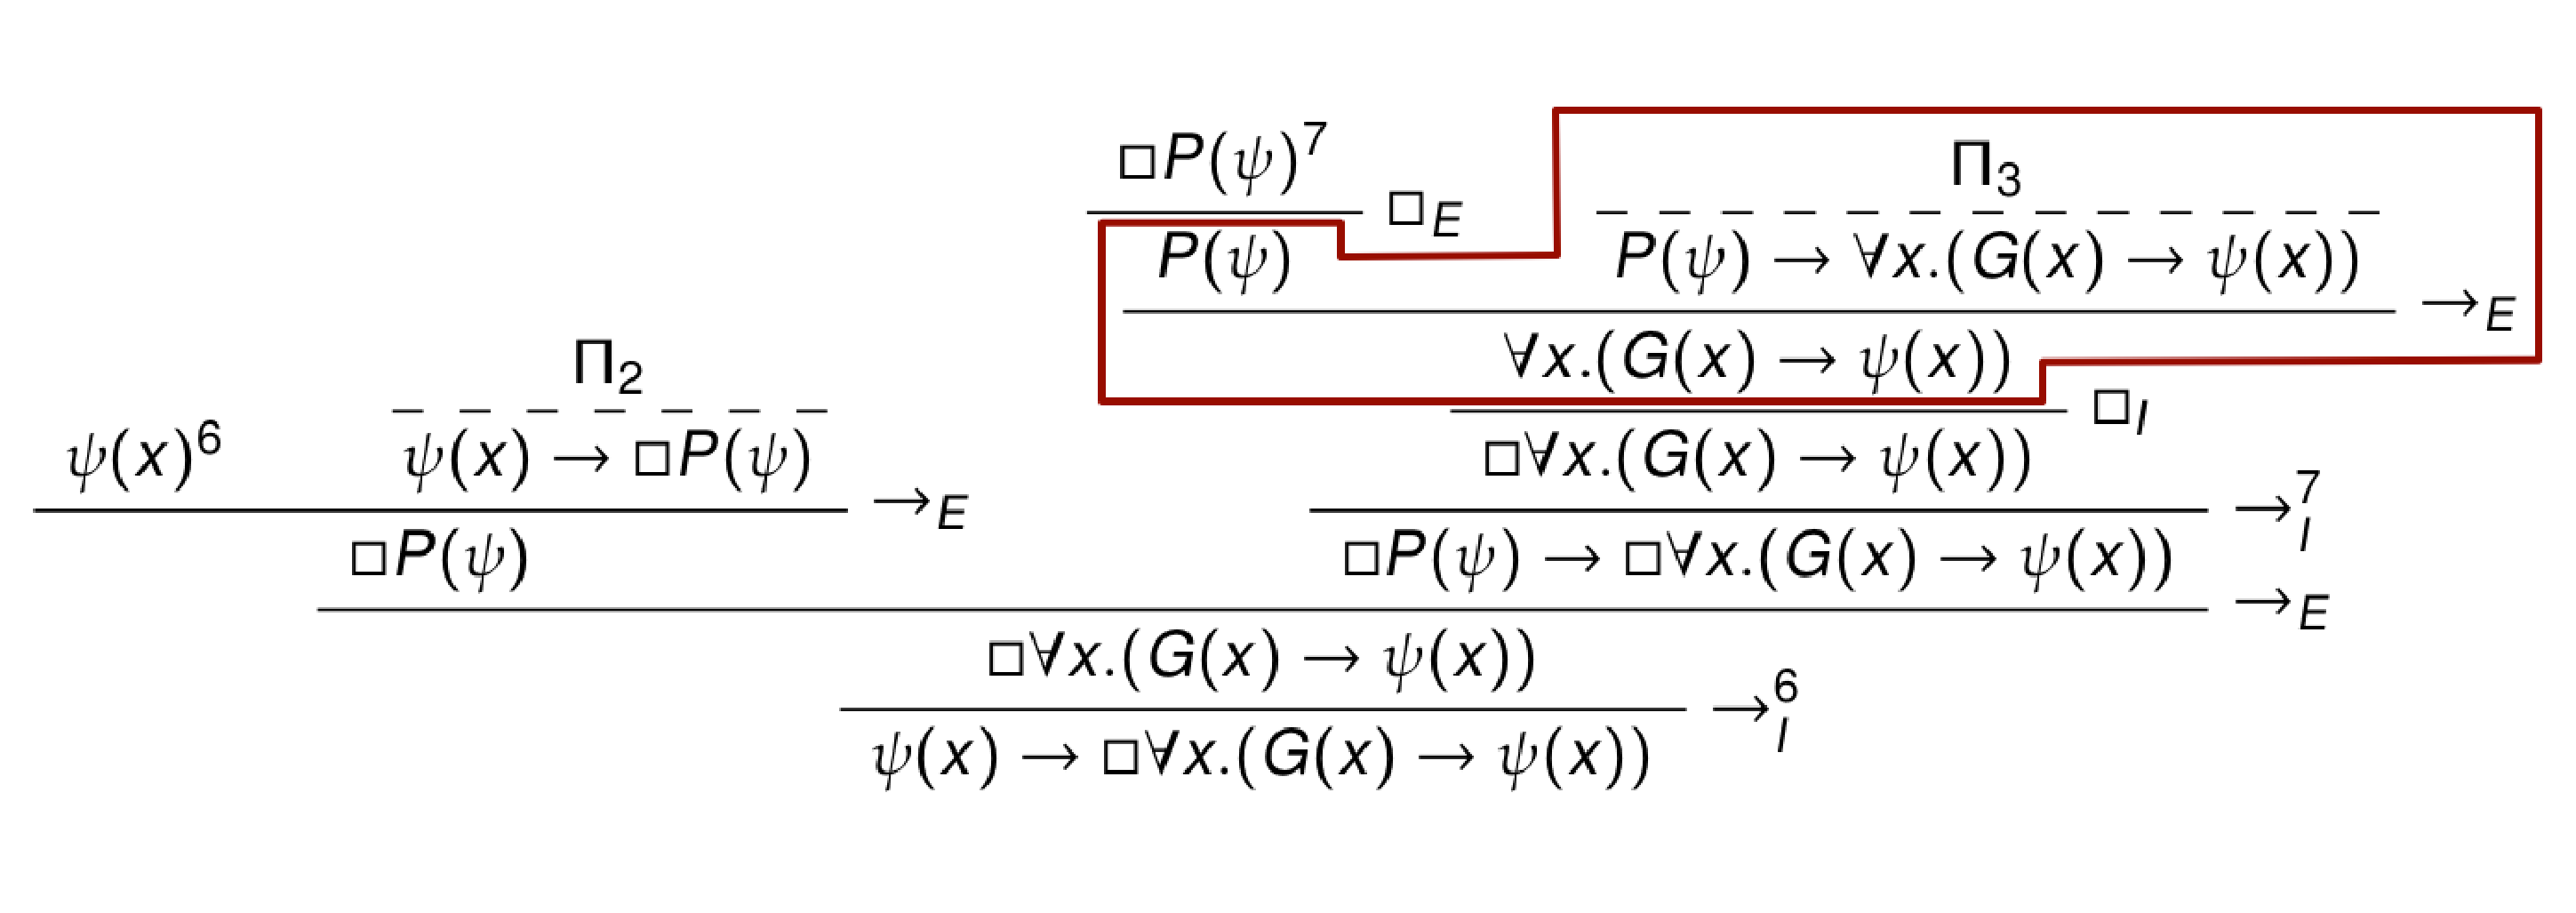
\includegraphics[scale=0.22]{Images/ProofOfT2Boxed.pdf}%$
\end{frame}


\begin{frame}{Implementations and Experiments}\Large
\begin{itemize}
\item Formal encodings (in HOL) of:
\begin{itemize}
\item modal logic axioms
\item axioms, definitions, and theorems in Scott's proof script
\end{itemize}
\item Experiments using automated provers
\begin{itemize} 
\item LEO-II, Satallax, AgsyHOL
\end{itemize}
\item Interactive proofs using proof assistants 
\begin{itemize}
\item Isabelle and Coq
\end{itemize}
\end{itemize}
\vfill
Source files available at:
\begin{center}
\url{https://github.com/FormalTheology/GoedelGod/}
\end{center}

\pause

\medskip

\alert{Demos on request!}
\end{frame}

\begin{frame}[t]{Results} \Large
\begin{itemize}
\onslide*<1->{\item Axioms and definitions are consistent.}
\onslide*<2->{\item Logic K is sufficient for proving T1, C and T2.}
\onslide*<2->{\item Logic KB is sufficient for proving the final theorem T3.}

\onslide*<3>{\vfill\centering
\colorbox{yellow}{
\begin{minipage}{.9\textwidth}
Adresses criticisms: modal logic S5 is too strong
$$
\all P.[ \pos \nec P \imp \nec P ] 
$$
If something is possibly necessary, then it is necessary.
% $$\pos\nec (A \vee \neg A)\qquad \nec(A \vee \neg A)$$

\bigskip

\alert{S5 usually considered adequate}

\textcolor{blue}{(But KB is sufficient! --- shown by HOL ATPs)}
$$
\all P.[ P \imp \nec \pos P ] 
$$
If something is the case, then it is necessarily possible.
\end{minipage}}}

\onslide*<4->{\item HOL-ATPs prove T1, C, and T2 from axioms quickly; \\
succeed in proving T3 from axioms, C and T2; \\
but fail in proving T3 from axioms alone. }
\onslide*<5->{\item G\"odel's original axioms and definitions,
  omitting conjunct $\phi(x)$ in the definition of \emph{essence}, 
  seem inconsistent.}
\onslide*<6->{\item $\ex x. G(x)$ can be proved without first proving $\nec \ex x. G(x)$.}
\onslide*<7->{\item Equality is not necessary to prove T1.}
\onslide*<8->{\item A2 may be used only once to prove T1.}
\end{itemize}
\end{frame}

\begin{frame}[t]{Results} \Large
\begin{itemize}
\onslide*<1->{\item G{\"o}del's axioms imply the \emph{modal collapse}:
  $\all \phi. (\phi \supset\Box\phi)$} 
\end{itemize}

\onslide*<2->{\vfill\centering
\colorbox{yellow}{
\begin{minipage}{.9\textwidth}
\begin{small}
Fundamental criticism against G{\"o}del's argument. \\[1em]
Everything that is the case is so necessarily.\\[1em]
Follows from T2, T3 and D2 \textcolor{blue}{(as shown by HOL ATPs)}.\\[1em]
There are no contingent ``truths''. \\
Everything is determined. \\
There is no free will. \\[1em]
Many proposed solutions: Anderson, Fitting, H\'ajek, \ldots
\end{small}
\end{minipage}}
}

\onslide*<3>{
\centering
\begin{figure}
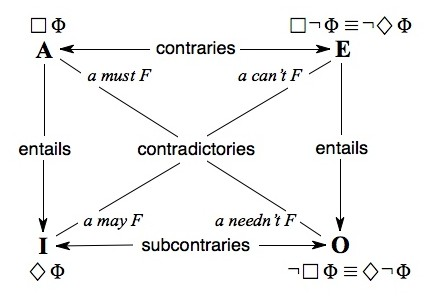
\includegraphics[width=0.4 \textwidth]{Images/ModalSquare}
\end{figure}
}

\end{frame}

\begin{frame}[t]{Results} \Large
\begin{itemize}
% \item For proving T1, only the $\supset$-direction of A1 is
%   needed. Some proposals try to avoid modal collapse by
%   replacing the $\supset$-direction of A1. However, the $\subset$-direction of A1 is required for proving T2. 
% \pause
\item God is \emph{flawless}: $\all x. G(x) \imp (\all \varphi. \neg P(\varphi) \imp \neg \varphi(x))$.
\pause
\item \emph{Monotheism}: $ \all x. \all y. G(x) \wedge G(y) \imp x=y$. % MT can
  % easily be proved by Satallax from FG and D1. It remains non-trivial
  % to prove it directly from G{\"o}del's axioms.
\end{itemize}

\pause
\centering
\vfill

All results hold for both \\
- constant domain semantics \\
- varying domain semantics

\end{frame}




\begin{transitionframe}{Images/Transitions/ComputerCross.png}{black}%$
\textbf{Conclusions}
\end{transitionframe}





% \begin{frame}{Summary of Results} \large

% Our novel contributions to the theorem proving community include \\[.5em]
% \begin{itemize}
% \item Powerful infrastructure for reasoning with QML
% \item A new natural deduction calculus for higher-order modal logic
% \item Difficult new benchmarks problems for HOL provers
% \item Huge media attention
% \end{itemize}
% \end{frame}

\begin{frame}{Conclusion} \large
\vskip-1em Achievements: \\[.5em]
\begin{itemize}
\item Infra-structure for automated higher-order modal reasoning
\item Verification of G\"odel's ontological argument with HOL provers
  \begin{itemize}
  \item experiments with different parameters
  \end{itemize}
\item Novel results and insights
\item Major step towards \alert{Computer-assisted Theoretical Philosophy}
 \begin{itemize}
  \item see also Ed Zalta's \emph{Computational Metaphysics} project at Stanford University
  \item see also John Rushby's recent verification of Anselm's proof in PVS
  \item remember Leibniz' dictum --- \emph{Calculemus!}
  \end{itemize}
\item Interesting bridge between CS, Philosophy and Theology
\end{itemize}

\pause

\vfill
\vskip-1em Ongoing and future work \\[.5em]
\begin{itemize}
\item Formalize and verify literature on ontological arguments
  \begin{itemize}
  \item \ldots in particular the criticisms and proposed improvements
  \end{itemize}
\item Own contributions --- supported by theorem provers
\end{itemize}
\end{frame}


\end{document}
